
\documentclass[12pt,a4paper]{article}
\usepackage[utf8]{inputenc}
\usepackage{amsmath}
\usepackage{amsfonts}
\usepackage{amssymb}
\usepackage{graphicx}
\usepackage{hyperref}
\usepackage{listings}
\usepackage{xcolor}

\definecolor{codegreen}{rgb}{0,0.6,0}
\definecolor{codegray}{rgb}{0.5,0.5,0.5}
\definecolor{codepurple}{rgb}{0.58,0,0.82}
\definecolor{backcolour}{rgb}{0.95,0.95,0.92}

\lstdefinestyle{mystyle}{
    backgroundcolor=\color{backcolour},   
    commentstyle=\color{codegreen},
    keywordstyle=\color{magenta},
    numberstyle=\tiny\color{codegray},
    stringstyle=\color{codepurple},
    basicstyle=\ttfamily\footnotesize,
    breakatwhitespace=false,         
    breaklines=true,                 
    captionpos=b,                    
    keepspaces=true,                 
    numbers=left,                    
    numbersep=5pt,                  
    showspaces=false,                
    showstringspaces=false,
    showtabs=false,                  
    tabsize=2
}

\lstset{style=mystyle}

\title{Scientific Calculator Implementation Report}
\author{EE24BTECH11038-M.B.S Aravind}
\date{\today}

\begin{document}

\maketitle

\begin{abstract}
This report documents the implementation of a scientific calculator using an Arduino microcontroller, LCD display, and push buttons. The calculator supports basic arithmetic operations, trigonometric functions, and multi-step calculations. The implementation demonstrates concepts of embedded systems programming, user interface design, and mathematical function implementation in resource-constrained environments.
\end{abstract}

\tableofcontents
\newpage

\section{Introduction}
The scientific calculator project aims to develop a fully functional calculator with numerical input capabilities and scientific functions. Unlike basic calculators, this implementation supports trigonometric functions (sine, cosine, tangent, and their inverse functions) along with standard arithmetic operations.

\section{Hardware Components}
The hardware implementation consists of the following components:
\begin{itemize}
    \item Arduino board (ATmega328P-based)
    \item 16x2 LCD display
    \item Breadboard
    \item Push buttons (14 total):
    \begin{itemize}
        \item 10 buttons for digits 0-9
        \item 1 button for operator cycling (+, -, *, /)
        \item 1 button for trigonometric function cycling (sin, cos, tan, asin, acos, atan)
        \item 1 button for decimal point
        \item 1 button for equals/enter
    \end{itemize}
    \item Jumper wires
    \item Resistors for button pull-ups (if not using internal pull-ups)
    \item Potentiometer
\end{itemize}

\section{LCD}
A Liquid Crystal Display (LCD) is an electronic display module used in embedded systems for visual representation of characters, numbers, and symbols. The 16x2 LCD module is one of the most commonly used displays in microcontroller-based projects.

\section{Features of 16x2 LCD}
The 16x2 LCD has the following key features:
\begin{itemize}
    \item Display: 16 characters per row, 2 rows
    \item Interface: Parallel (4-bit or 8-bit mode)
    \item Power Supply: 5V DC
    \item Backlight: LED backlight for better visibility
    \item Control Pins:
    \begin{itemize}
        \item \textbf{RS (Register Select)}: Chooses command or data mode
        \item \textbf{RW (Read/Write)}: Selects read or write operation (often tied to ground for write-only operation)
        \item \textbf{E (Enable)}: Latches the command/data into the LCD
    \end{itemize}
\end{itemize}

\section{Pin Configuration}
The 16x2 LCD has 16 pins with the following functions:
\begin{table}[h]
    \centering
    \begin{tabular}{|c|c|c|}
        \hline
        Pin No. & Name & Function \\
        \hline
        1 & VSS & Ground (0V) \\
        2 & VCC & Power Supply (5V) \\
        3 & VEE & Contrast Adjustment \\
        4 & RS & Register Select \\
        5 & RW & Read/Write Control \\
        6 & E  & Enable Signal \\
        7-14 & D0-D7 & Data Pins \\
        15 & LED+ & Backlight Positive \\
        16 & LED- & Backlight Negative \\
       \hline
    \end{tabular}
    \caption{16x2 LCD Pin Configuration}
    \label{tab:lcd_pins}
\end{table}

\section{Circuit Diagram}
Below is the circuit diagram for interfacing a 16x2 LCD with an Arduino:\\

\begin{figure}[h]
    \centering
    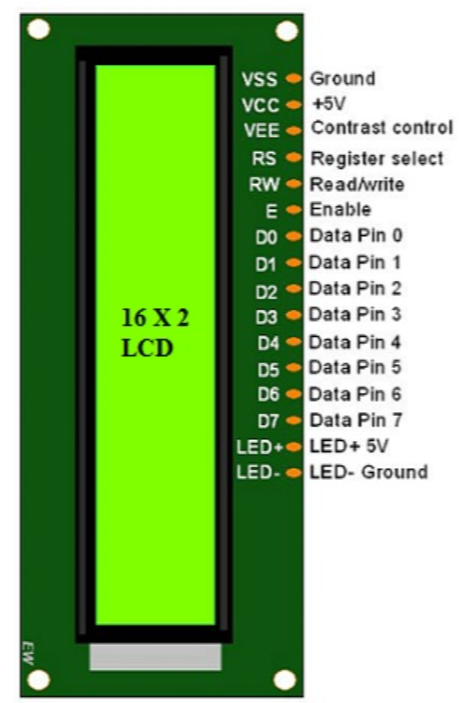
\includegraphics[width=0.5\textwidth]{LCD display.png} % Replace with actual file name
    \caption{Interfacing 16x2 LCD with Arduino}
    \label{fig:lcd_circuit}
\end{figure}\\

\section{Working Principle}
The LCD operates using liquid crystal molecules that align in response to an electric field to control the passage of light. It requires initialization commands before displaying data. It supports both **4-bit and 8-bit communication**, with **4-bit mode** reducing the number of GPIO pins used.
\section{Hardware Configuration}
\subsection{LCD Connection}
The LCD is connected to the Arduino using a 4-bit interface to save I/O pins:
\begin{itemize}
    \item RS (Register Select): Arduino pin 1 (PD1)
    \item E (Enable): Arduino pin 0 (PD0)
    \item D4: Arduino pin 5 (PD5)
    \item D5: Arduino pin 4 (PD4)
    \item D6: Arduino pin 3 (PD3)
    \item D7: Arduino pin 2 (PD2)
\end{itemize}

\subsection{Button Connections}
The buttons are connected to Arduino pins as follows:
\begin{itemize}
    \item Digit 0: Arduino pin 13 (PB5)
    \item Digit 1: Arduino pin 12 (PB4)
    \item Digit 2: Arduino pin 11 (PB3)
    \item Digit 3: Arduino pin 10 (PB2)
    \item Digit 4: Arduino pin 9 (PB1)
    \item Digit 5: Arduino pin 8 (PB0)
    \item Digit 6: Arduino pin 7 (PD7)
    \item Digit 7: Arduino pin 6 (PD6)
    \item Digit 8: Arduino pin A0 (PC0)
    \item Digit 9: Arduino pin A1 (PC1)
    \item Operator: Arduino pin A2 (PC2)
    \item Trig Function: Arduino pin A3 (PC3)
    \item Decimal Point: Arduino pin A4 (PC4)
    \item Enter/Equals: Arduino pin A5 (PC5)
\end{itemize}

\begin{figure}[h]
    \centering
    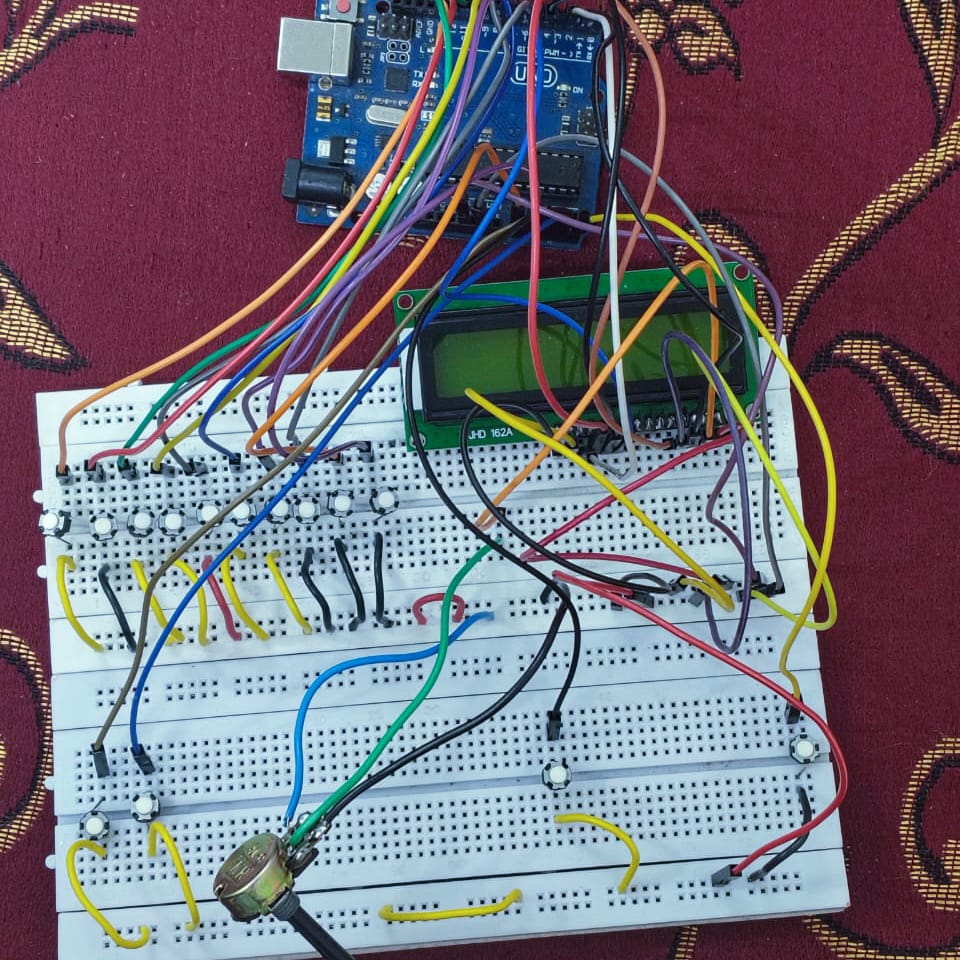
\includegraphics[width=0.5\textwidth]{circuit.jpeg} % Replace with actual file name
    
    \label{fig:lcd_circuit}
\end{figure}\\
\section{Software Design}
\subsection{Software Architecture}
The calculator software is structured around the following key components:
\begin{itemize}
    \item LCD Interface: Functions to initialize and communicate with the LCD
    \item Button Interface: Functions to initialize buttons and detect button presses
    \item Expression Parser: Functions to build and evaluate mathematical expressions
    \item Mathematical Functions: Implementation of trigonometric functions
\end{itemize}

\subsection{Key Data Structures}
\begin{itemize}
    \item \texttt{expression[32]}: Character array to store the current expression
    \item \texttt{exprIndex}: Index for the current position in the expression string
    \item \texttt{operation}: Current selected arithmetic operation
    \item \texttt{trigMode}: Current selected trigonometric function
    \item \texttt{lastResult}: Stores the last calculated result for continued operations
\end{itemize}

\subsection{Expression Evaluation}
The calculator uses a recursive descent parser to evaluate mathematical expressions. The implementation:
\begin{itemize}
    \item Handles parentheses and nested expressions
    \item Maintains correct operator precedence
    \item Processes expressions from left to right
    \item Handles trigonometric functions and their arguments
\end{itemize}

\subsection{User Interface Design}
The UI is designed for simplicity and usability with limited buttons:
\begin{itemize}
    \item The LCD displays the current expression and results
    \item The operator button cycles through +, -, *, and /
    \item The trig button cycles through sin, cos, tan, asin, acos, and atan
    \item The decimal button adds a decimal point to the current number
    \item The enter button evaluates the expression and displays the result
\end{itemize}

\section{Implementation Challenges}
Several challenges were addressed during implementation:
\subsection{Limited Memory}
The Arduino's limited memory required efficient string handling and expression evaluation:
\begin{itemize}
    \item Optimized string functions to reduce memory usage
    \item Implemented a custom expression evaluator instead of using library functions
    \item Limited expression length to 32 characters
\end{itemize}

\subsection{Expression Parsing}
Implementing a correct expression parser required addressing:
\begin{itemize}
    \item Order of operations for mathematical expressions
    \item Handling of nested parentheses
    \item Proper handling of trigonometric functions
    \item Error detection and handling (e.g., division by zero)
\end{itemize}

\subsection{User Interface Limitations}
With limited buttons, the interface required innovative solutions:
\begin{itemize}
    \item Cycling through operators with a single button
    \item Cycling through trigonometric functions with a single button
    \item Clear feedback on the current state through the LCD display
    \item Handling of continuing calculations from previous results
\end{itemize}

\section{Software Functional Blocks}
\subsection{LCD Control Functions}
These functions handle all LCD communication:
\begin{itemize}
    \item \texttt{lcd\_init()}: Initializes the LCD
    \item \texttt{lcd\_send\_command()}: Sends a command to the LCD
    \item \texttt{lcd\_send\_data()}: Sends data to the LCD
    \item \texttt{lcd\_clear()}: Clears the LCD display
    \item \texttt{lcd\_set\_cursor()}: Sets the cursor position
    \item \texttt{lcd\_print()}: Displays a string on the LCD
\end{itemize}

\subsection{Button Interface Functions}
These functions manage button input:
\begin{itemize}
    \item \texttt{init\_buttons()}: Sets up button pins
    \item \texttt{check\_button()}: Checks if a specific button is pressed
\end{itemize}

\subsection{Expression Handling Functions}
These functions manage the mathematical expression:
\begin{itemize}
    \item \texttt{append\_char()}: Adds a character to the expression
    \item \texttt{append\_string()}: Adds a string to the expression
    \item \texttt{append\_operator()}: Handles operator input
    \item \texttt{append\_trig\_function()}: Handles trigonometric function input
\end{itemize}

\subsection{Calculation Functions}
These functions perform the mathematical calculations:
\begin{itemize}
    \item \texttt{evaluate\_expression()}: Evaluates a mathematical expression
    \item \texttt{process\_enter()}: Processes the enter button press
    \item \texttt{balance\_parentheses()}: Ensures all parentheses are balanced
\end{itemize}

\section{Testing Results}
\subsection{Arithmetic Operations}
Tests were conducted to verify the correct operation of basic arithmetic:
\begin{table}[h]
\centering
\begin{tabular}{|l|l|l|}
\hline
\textbf{Expression} & \textbf{Expected Result} & \textbf{Actual Result} \\
\hline
2 + 3 & 5 & 5 \\
\hline
5 - 2 & 3 & 3 \\
\hline
4 * 3 & 12 & 12 \\
\hline
10 / 2 & 5 & 5 \\
\hline
2 + 3 * 4 & 14 & 14 \\
\hline
\end{tabular}
\caption{Arithmetic operation test results}
\end{table}

\subsection{Trigonometric Functions}
Tests were conducted to verify the correct operation of trigonometric functions:
\begin{table}[h]
\centering
\begin{tabular}{|l|l|l|}
\hline
\textbf{Expression} & \textbf{Expected Result} & \textbf{Actual Result} \\
\hline
sin(30) & 0.5 & 0.5 \\
\hline
cos(60) & 0.5 & 0.5 \\
\hline
tan(45) & 1.0 & 1.0 \\
\hline
asin(0.5) & 30.0 & 30.0 \\
\hline
acos(0.5) & 60.0 & 60.0 \\
\hline
atan(1.0) & 45.0 & 45.0 \\
\hline
\end{tabular}
\caption{Trigonometric function test results}
\end{table}

\section{Limitations and Future Improvements}
\subsection{Current Limitations}
\begin{itemize}
    \item Expression length limited to 32 characters
    \item Limited input method requires cycling through operators and functions
    \item No memory functions (store/recall)
    \item Limited error handling and reporting
    \item No parentheses input button (parentheses only added by trig functions)
\end{itemize}

\subsection{Potential Improvements}
\begin{itemize}
    \item Add a backspace/delete function
    \item Implement memory functions (M+, MR, MC)
    \item Add more scientific functions (logarithmic, exponential)
    \item Implement a better error reporting system
    \item Add dedicated parentheses buttons
    \item Use a larger LCD display for better visibility
    \item Implement a more efficient parsing algorithm
\end{itemize}

\section{Conclusion}
The scientific calculator implementation successfully demonstrates a functional calculator with both basic arithmetic and trigonometric capabilities. Despite the limitations of the Arduino platform and the minimal input interface, the calculator provides accurate calculations and a usable interface.

The project showcases embedded systems programming techniques, mathematical expression parsing, and user interface design with limited resources. The modular code structure allows for future extensions and improvements.

\appendix
\section{Code Highlights}
\subsection{Expression Evaluation Function}
This is the core function that evaluates mathematical expressions:
\section{Pin Assignment Table}
\begin{table}[h]
\centering
\begin{tabular}{|l|l|l|}
\hline
\textbf{Component} & \textbf{Arduino Pin} & \textbf{AVR Port/Pin} \\
\hline
LCD RS & 1 & PD1 \\
\hline
LCD E & 0 & PD0 \\
\hline
LCD D4 & 5 & PD5 \\
\hline
LCD D5 & 4 & PD4 \\
\hline
LCD D6 & 3 & PD3 \\
\hline
LCD D7 & 2 & PD2 \\
\hline
Button 0 & 13 & PB5 \\
\hline
Button 1 & 12 & PB4 \\
\hline
Button 2 & 11 & PB3 \\
\hline
Button 3 & 10 & PB2 \\
\hline
Button 4 & 9 & PB1 \\
\hline
Button 5 & 8 & PB0 \\
\hline
Button 6 & 7 & PD7 \\
\hline
Button 7 & 6 & PD6 \\
\hline
Button 8 & A0 & PC0 \\
\hline
Button 9 & A1 & PC1 \\
\hline
Operator Button & A2 & PC2 \\
\hline
Trig Button & A3 & PC3 \\
\hline
Decimal Button & A4 & PC4 \\
\hline
Enter Button & A5 & PC5 \\
\hline
\end{tabular}
\caption{Pin assignment table}
\end{table}

\end{document} 
